\section{Smart Cards}
\begin{center}
\begin{tikzpicture}
\draw [rounded corners=15pt, firstAccent] (0,0) rectangle (4,3);

\draw [firstAccent] (0, 0.8) -- (0.3, 0.8) -- (0.3, 0.3) -- (1.7, 0.3) --(1.7, 1.2) -- (0, 1.2);
\draw [firstAccent] (0, 2.2) -- (0.3, 2.2) -- (0.3, 2.7) -- (1.7, 2.7) -- (1.7, 1.8) -- (0, 1.8);
\node (2) at (0, 1.5) [draw, anchor=west, rounded rectangle, rounded  rectangle west arc=0pt, minimum height=1cm, minimum width=1.5cm, firstAccent, fill=white] {};
\draw [firstAccent] (0, 1.5) -- (1.25, 1.5);

\draw [firstAccent] (4, 0.8) -- (3.7, 0.8) -- (3.7, 0.3) -- (2.3, 0.3) --(2.3, 1.2) -- (4, 1.2);
\draw [firstAccent] (4, 2.2) -- (3.7, 2.2) -- (3.7, 2.7) -- (2.3, 2.7) -- (2.3, 1.8) -- (4, 1.8);
\node (2) at (4, 1.5) [draw, anchor=east, rounded rectangle, rounded  rectangle east arc=0pt, minimum height=1cm, minimum width=1.5cm, firstAccent, fill=white] {};
\draw [firstAccent] (2.75, 1.5) -- (4, 1.5);


\node (EP) at (2, 4) [draw, anchor=south] {External power, 3-5 V};
\node (Vcc) at (1, 3.3) [draw, anchor=south] {Vcc};
\node (GND) at (3, 3.3) [draw, anchor=south] {GND};
\draw (Vcc |- EP.south) -- (Vcc);
\draw (GND |- EP.south) -- (GND); 
\draw (Vcc) -- (1, 2.25); 
\draw (GND) -- (3, 2.25); 

\node (RST) at (-0.3, 1.8) [draw, anchor=east] {RST};
\node (CLK) at (-0.3, 1.2) [draw, anchor=east] {CLK, 3.5-5 MHz};
\draw (RST) -- (0.5, 1.8);
\draw (CLK) -- (0.5, 1.2);

\node (USB) at (2, -0.3) [draw, anchor=north] {USB signaling};
\draw (USB) |- (1, 0.75);
\draw (USB) |- (3, 0.75); 

\node (EPROM) at (4.3, 1.8) [draw, anchor=west] {EEPROM};
\node (IO) at (4.3, 1.2) [draw, anchor=west] {I/O};
\draw (EPROM) -- (3.5, 1.8);
\draw (IO) -- (3.5, 1.2);

\end{tikzpicture}
\captionof{figure}{Smart card ISO standard}
\end{center}
\begin{mytitle}[Main use] Smart cards are portable secure containers for secret data. They are a secure environment for cryptographic algorithms, but they are also interesting for ubicomp technology because they are a cheap, small and disposable computer with security tokens. 
\end{mytitle}
\begin{mytitle}[Memory cards vs processor cards] Memory cards are just a container for data, usually with access control for parts of the memory. They are cheap (around 1 euro) but not truly smart. Processor cards on the other hand have an internal microprocessor and RAM. They optionally contain a true random generator or hardware crypto-functionality. Processor cards cost 1 - 20 euros.
\end{mytitle}
\begin{center}
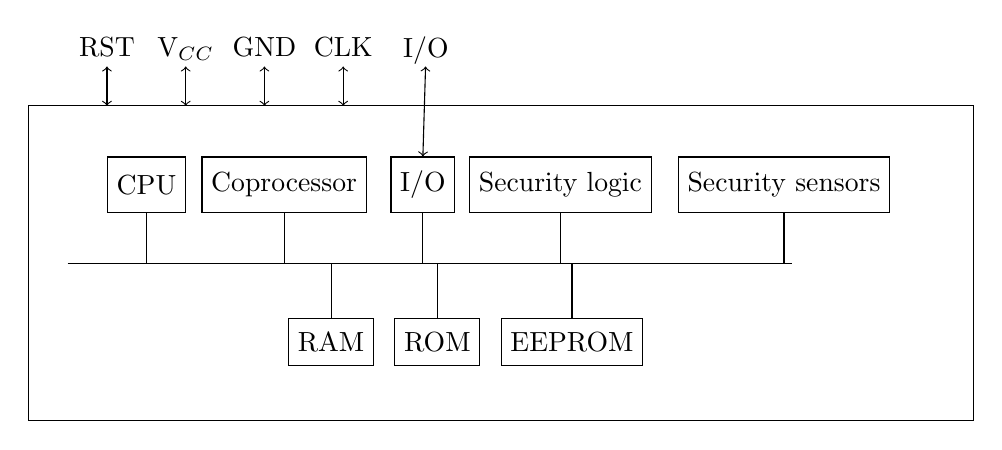
\begin{tikzpicture}
\draw [] (-1,-2) rectangle (11,2);
\node (CPU) at (0,1) [draw, anchor=west, minimum height=0.7cm] {CPU};
\node (Co) at (1.2,1) [draw, anchor=west, minimum height=0.7cm] {Coprocessor};
\node (IO) at (3.6,1) [draw, anchor=west, minimum height=0.7cm] {I/O};
\node (SL) at (4.6,1) [draw, anchor=west, minimum height=0.7cm] {Security logic};
\node (SS) at (7.25,1) [draw, anchor=west, minimum height=0.7cm] {Security sensors};

\draw (-0.5,0) -- (8.7, 0);
\node (line) at (-0.5,0) [anchor=west, minimum width=9cm] {};

\node (RAM) at (2.3,-1) [draw, anchor=west, minimum height=0.6cm] {RAM};
\node (ROM) at (3.65,-1) [draw, anchor=west, minimum height=0.6cm] {ROM};
\node (EEPROM) at (5,-1) [draw, anchor=west, minimum height=0.6cm] {EEPROM};

\draw (CPU.south |- line) -- (CPU);
\draw (Co.south |- line) -- (Co);
\draw (IO.south |- line) -- (IO);
\draw (SL.south |- line) -- (SL);
\draw (SS.south |- line) -- (SS);
\draw (RAM.north |- line) -- (RAM);
\draw (ROM.north |- line) -- (ROM);
\draw (EEPROM.north |- line) -- (EEPROM);

\node (RST) at (0, 2.5) [anchor=south] {RST};
\draw [<->](RST) -- (0, 2);
\node (VCC) at (1, 2.45) [anchor=south] {V$_{\text{CC}}$};
\node (VCC2) at (1, 2.5) [anchor=south] {};
\draw [<->](VCC2) -- (1, 2);
\node (GND) at (2, 2.5) [anchor=south] {GND};
\draw [<->](GND) -- (2, 2);
\node (CLK) at (3, 2.5) [anchor=south] {CLK};
\draw [<->](CLK) -- (3, 2);
\node (IO2) at (4.05, 2.4) [anchor=south] {I/O};
\node (IO3) at (4.05, 2.5) [anchor=south] {};
\draw [<->](IO3) -- (IO.north);

\end{tikzpicture}
\captionof{figure}{Processor Card}
\end{center}
\begin{mytitle}[Random number generation (RNG)] There are two types of RNGs:
\begin{itemize}
    \item Pseudo random numbers are typically generated based on some logical CPU states that are incremented by a clock or a crypto-algorithm such as DES.
    \item True random number generators exploit physical characteristics (i.e. noise).
\end{itemize}
\end{mytitle}
\begin{mytitle}[Communication with the card] Communication between the card reader and the smart card is always initiated by the reader. The card gets Vcc and CLK and does a ``reset''. Within a few ms, it sends back an ``answer to reset'' (ATR) containing basic information about the card. Then the terminal sends the first command application protocol data unit (APDU) to the card and the card answers with a response APDU. Encryption and authentication is possible, but slows down the communication by a factor of 4.
\end{mytitle}
\begin{mytitle}[Subscriber identity module (SIM)] The SIM is the security module for accessing the mobile phone network.
\end{mytitle}
\begin{mytitle}[Contact-less smart cards] These smart cards use an external energy source like RFID does. They are more expensive but have better security compared to RFID tags.
\end{mytitle}
\begin{myremark} The secret data inside the card must never leave the card and computations must not be observable from the outside.
\end{myremark}
\begin{mytitle}[Entity authentication] \hfill
\begin{itemize}
    \item Internal authentification: The terminal verifies the card by sending a random number to the card to be hashed/encrypted using a key. The card provides the hash/ciphertext, with that the terminal knows that the card is authentic.
    \item External authentification: The card verifies the terminal for which the terminal first asks for a challenge which the card provides. The card can then analyze the response to know that the terminal is authentic. 
    \item Card holder authentification: The terminal asks the user to provide the password and sends it to the card for verification.
\end{itemize} 
\end{mytitle}
\subsection{Smart Card Components}
\begin{mytitle}[Smart card hardware] The typical hardware has cheap classical 8 bit and 16 bit processors, a memory management unit (MMU) necessary for multi-application smart cards and 1 - 10 MHz externally supplied power.
\end{mytitle}
\begin{mytitle}[Smart card operating system] The typical operating systems is smaller than 100 kB and very simple with no user interface, no external devices, no interrupts and no multiprogramming but security is of prime importance. It is highly dependent on the hardware. Access to the operating system functions via an API.
\end{mytitle}
\begin{mytitle}[Smart card instructions] There exist several standards that define instructions. Some examples of instruction types are file operations (select, read, write, seek, \ldots), security (authentication and encryption), application specific operations (e.g. instructions for an electronic purse) and operations for testing.
\end{mytitle}
\begin{mytitle}[Smart card file system] Smart cards use a hierarchical file system in EEPROM. There has to be support for different types of files and several types of access control, as well as file access commands like create, delete, write, read, append, lock, invalidate and seek.
\end{mytitle}
\newpage
\subsection{Attacks}
\begin{mytitle}[Attack classification] There are three kinds of attackers:
\begin{itemize}
    \item Clever outsiders: they use existing weaknesses in systems
    \item Knowledgeable insiders: they have access to highly sophisticated tools
    \item Funded organizations: they have virtually unlimited resources
\end{itemize}
\end{mytitle}
\begin{mytitle}[Leakage] Power consumption, heat, electromagnetic emissions, timing and faulty outputs are all side-channel information that get leaked and can be used in attacks.
\end{mytitle}
\begin{mytitle}[Simple attacks]\hfill
\begin{itemize}
    \item Clock bursts: momentarily cause a rapid increase in the clock frequency, this causes instructions to be skipped
    \item Voltage glitch: momentarily cause a drop in voltage, this causes instructions to be decoded incorrectly
    \item Acid hacking: gain access to ROM by physically gaining access to see the bits. One could then simply read out from the memory. Another possible use is the  manipulation of the random generator so that it always yields the same number. Again another use is to set the bit of an unknown secret key to 0 or 1, the application will then typically return a parity error if the guess was incorrect. 
\end{itemize}
\end{mytitle}
\begin{mytitle}[More advanced attacks]\hfill
\begin{itemize}
    \item Power analysis attack: The attacker measures the power consumption to learn the bits of the secret key. When no special counter-measures are taken, this is applicable for almost all crypto-algorithms and smart cards.
    \item Hamming weight leakage: The attacker learns the number of 1s in each of the seven 8-bit words of the secret key by using an electromagnetic probe. This reduces the brute-force search space from $2^{56}$ to $2^{40}$. (That is a factor of 65'536.)
    \item Timing attack: Because there is code that is only executed when the bit is 1, the operation will take a bit longer in that case. From this information the attacker can also learn the bits of the secret key.
\end{itemize}
\end{mytitle}

\subsection{Counter-measures}
\begin{mytitle}[Hardware counter-measures] \hfill
\begin{itemize}
    \item Balance/equalize power consumption
    \item Increase noise
    \item Vary the execution time of instructions
    \item Randomly modify the internal clock speed
\end{itemize}
\end{mytitle}
\begin{mytitle}[Software counter-measures]\hfill
\begin{itemize}
    \item Add random instructions to desynchronize
    \item Don't let the timing depend on the data or the key
    \item Limit the number of times an algorithm can be executed
\end{itemize}
\end{mytitle}
\begin{mytitle}[General counter-measures]\hfill
\begin{itemize}
    \item Scramble the data bus and memory cells/addresses differently for each chip
    \item Use dual logic where 10 = low and 01 = high. They always consume the same amount of power.
    \item Use a dual CPU where the same operation is performed on two CPUs and then compared.
    \item Use checksums on memory content.
    \item Encrypt the memory content
    \item Encrypt/decrypt the data on the bus with dynamic random keys.
    \item Use shielding and protection layers
\end{itemize}
\end{mytitle}
\begin{mytitle}[Active hardware counter-measures]\hfill
\begin{itemize}
    \item Use sensors reacting to light, temperature sensors against increased clock rates and resistance/capacity sensors to detect removal of the chips protection layers.
    \item Watch the current and clock-frequency to detect hardware attacks.
    \item Do functional tests of parts of the chip.
    \item Overwrite critical parts of the EEPROM when an attack is suspected.
    \item Coat the chip with random particles with a high dielectric constant. An array of capacitive sensors detects those properties and uses them as secret random information.
\end{itemize}
\end{mytitle}